\chapter{Introduction}\label{ch1:introduction}
 
From pertinent work meetings to casual conversations with family and friends, an ever increasing number of people use applications like FaceTime, Zoom, and Google Meet, to name a few. One way of improving video chat experience is to bring in a feel of 3D by providing alternate views (images or frames) of each viewed scene rendered at different viewpoints. To fortify the 3D experience each novel view would have to be rendered at the right angle such that it aligns with the viewpoint of the viewer. This would require taking the viewer's transient head pose\footnote{In computer vision and robotics literature, the pose of an object generally refers to the combination of its position and orientation. In contrast, we only use the orientation of the viewer's head in 3D world space in rerendering viewed scenes.} into account.

\begin{figure}[!h]
    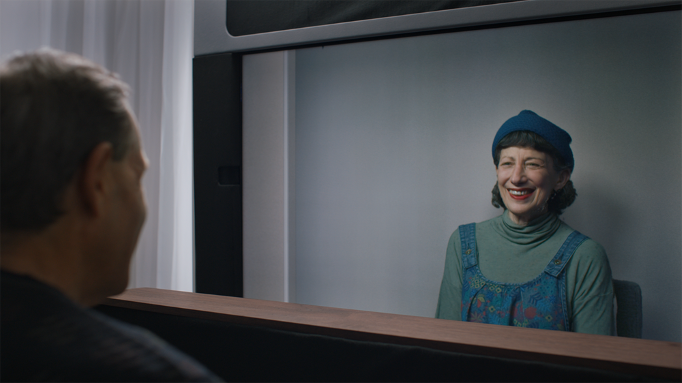
\includegraphics[width=1\columnwidth]{figures/google-starline-416.png}
    \caption{Google's Project Starline}
    \label{fig:google-starline}
    {\small Project Starline is expected to use a groundbreaking light field rendering system that would improve glasses-free 3D / automultiscopic video chat experience by leaps and bounds when it releases later this year.}
\end{figure}

Currently, synthesis of high-quality novel views is difficult to achieve end-to-end without some form of an intermediate representation of the structure (such as 3D world points) of the scene depicted by the given image(s). For instance, Google's Project Starline (Fig.~\ref{fig:google-starline}) uses a dense 3D representation to go from known views to novel views. One impressive variation of such an intermediate representation is called a Multiplane Image (MPI) --- first reintroduced in Zhou et al.~\cite{zhou2018stereo} (Fig.~\ref{fig:mpi-layered-representation}). It is a volumetric representation that reprojects the 2D points that make up an image onto multiple 2D planes situated one behind the other at successive depths along the z-axis, according to the computed alpha/transparency value at each point to be mapped. These MPI planes are parallel to each other and also to a reference coordinate frame centered at a reference camera/viewpoint looking down positive z-axis. The reference camera can be that of the image itself or of a different view of the scene captured by the image. One popular instance of such depth planes used in an MPI consists of a set of 32 planes positioned at equidistant disparity, with the near and far planes being at 1m and 100m, respectively, in 3D world space. Since disparity is inversely proportional to depth, the pixels on the nearer MPI planes are closer to the reference camera than the ones on the farther planes but they have greater disparity values associated with them then the farther ones.

\begin{figure}[!h]
    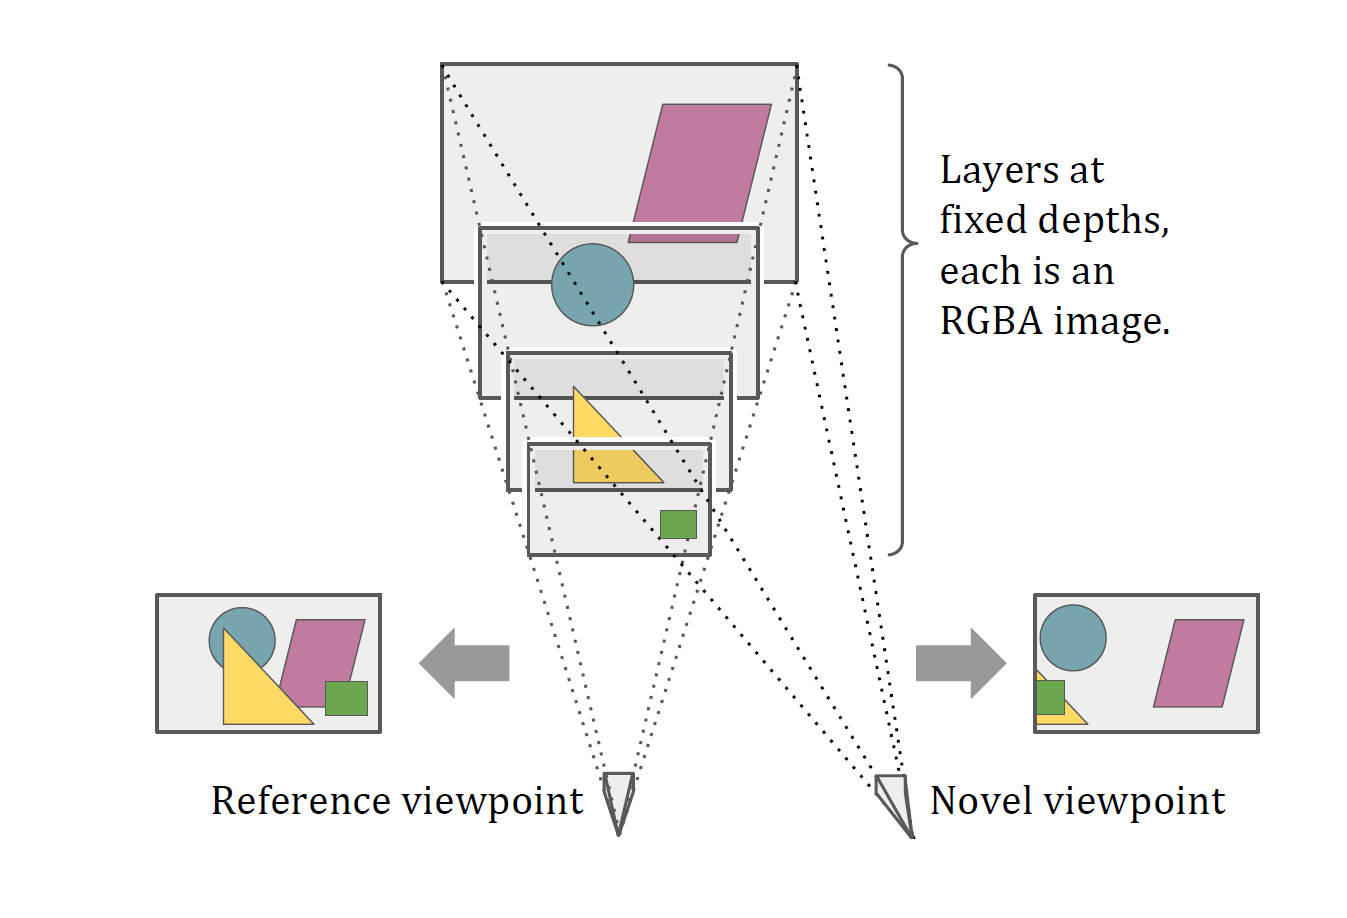
\includegraphics[width=1\columnwidth]{figures/mpi-layered-representation.png}
    \caption{The Volumetric/Layered MPI Representation}
    \label{fig:mpi-layered-representation}
    {\small A given image is reprojected onto multiple MPI planes with a common reference viewpoint that may or may not match with the given image's viewpoint. A novel image is synthesized by alpha-blending these intermediate layers in back-to-front order.}
\end{figure}

Disparity refers the number of pixels that each point in a image shifts over by in any of its warped/transformed counterparts that can relate to it via a homography (projective transform function). Disparity is required for triangulating the depth at each point of the image with respect to its warped version(s). Triangulating depth and estimating the 3D scene structure is easier when two or more of the scene's images are subjected to either stereo or multi-view image rectification, respectively. Such image rectification procedures typically involve rotating and shifting the optical centers of each image so they became collinear and scaling --- adjusting the focal lengths of the cameras of --- the images themselves so they become coplanar. Rectified image sets are characterized by point displacements only in the horizontal/row-wise $x$ direction. Properties of similar triangles can then be applied to the rectified images to get at the z-coordinate of each 3D world scene point most agreed upon by all the images containing the point's projections, after accounting for projection errors. Fig.~\ref{fig:disparity-triangulation} shows the triangulation process for a stereo pair. This is akin to how the human visual system (including the eyes, the ganglia therein, the dorsal and ventral streams of the brain, and the visual cortex) is able to triangulate depth from binocular vision. The brain is backed by prior knowledge, heuristics, and biases (made apparent by optical illusions) that it is able to use to infer depth to some degree of approximation even with one eye closed. Since Artificial Neural Networks (ANNs) are basically trying to replicate and someday even surpass the workings of the human brain, we are actually trying to fill in for this prior knowledge acquired by the brain by providing ANNs with copious amounts of data to learn from and devise their own heuristics. Therefore, in light of these facts, we may only generate an MPI for an image when we are provided either with one or more shifted and/or rotated reprojections of the scene in the image or the homographies for generating each of these transformed images from the original image. Otherwise, we would need to be supplied the sparse/dense 3D point cloud of the image's scene itself. 

\begin{figure}[!h]
    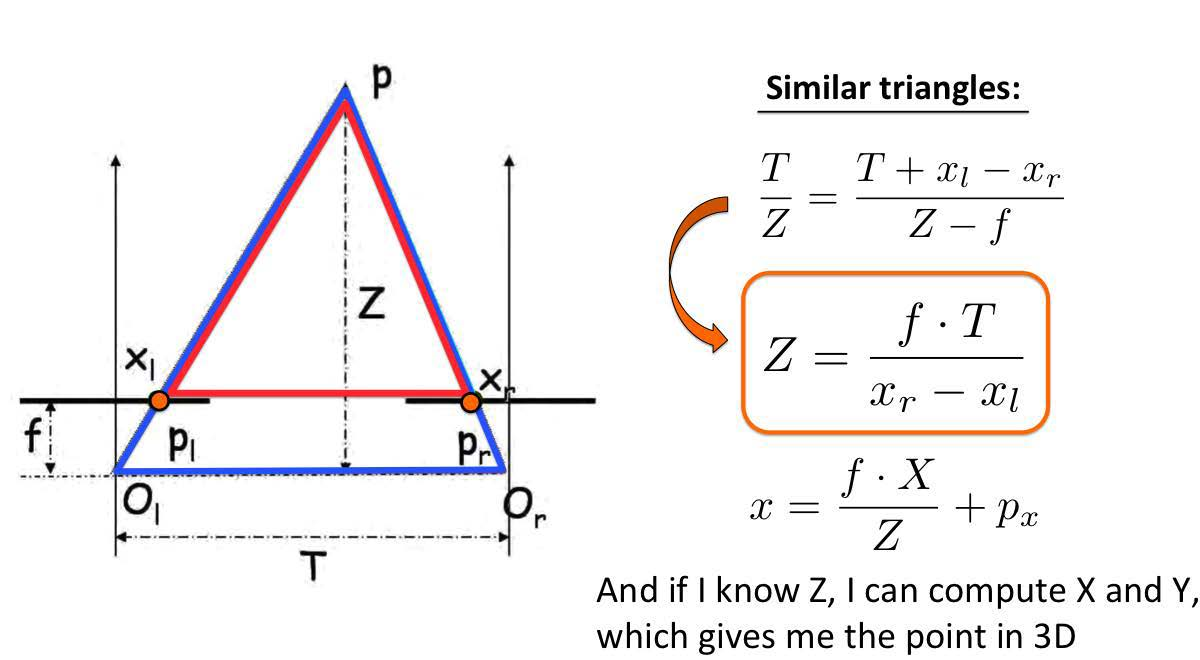
\includegraphics[width=1\columnwidth]{figures/disparity-triangulation.png}
    \caption{Disparity used in Triangulating 3D Points~\cite{fidler_depth_2021}}
    \label{fig:disparity-triangulation}
    {\small In this birds-eye view down the y-axis, $O_l$ and $O_r$ are the optical/camera centers of the left and right images of a stereo pair, $p_l$ and $p_r$ are the 2D projections of the same 3D world point $p$ onto the stereo pair, $x_l$ and $x_r$ are the x-coordinates of these 2D image points (y-coordinates are the same for corresponding points in a stereo pair), $f$ is the common focal length of the stereo cameras, $T$ is the horizontal translation or baseline of the stereo cameras, and $Z$ is the perpendicular depth of $p$ from the common reference coordinate frame of the stereo cameras and is inversely proportional to the disparity, $x_r - x_l$. Taking similar birds-eye perspectives down the $z$ and $x$ axes, we can compute the $x$ and $y$ coordinates of the 3D point as well.}
\end{figure}

To give a gist of our work, it began by attempting to retrain Tucker and Snavely's state-of-the-art end-to-end fully-convolutional single-view view synthesis with MPIs CNN~\cite{single_view_mpi} on the MannequinChallenge dataset. We hypothesized --- as was also hinted at in the paper --- that such retraining would be sufficient to generate high quality MPIs of scenes involving close-up shots of people typical of video chat settings. The original model is able to do the same for real estate scenes. We then went on to compare the inference results of this primary model variant with those of another variant trained on the MannequinChallenge dataset extended by the RealEstate10K dataset, taking the pretrained Tucker and Snavely model as baseline. This was so we could determine the best variant to apply to the domain of 3D video chat. Such application was by way of a two-way rendering of appropriate novel views of the concurrent dynamic scenes viewed by the participants of one-on-one video chats in both directions simultaneously. In the two-way pipeline, a novel view of a video frame is rendered every time a change in head pose is detected in the participant in the opposite frame. To our knowledge, MPIs have no been used in 3D video chat so far. We publish the code used to fill in the missing pieces of Tucker and Snavely's training and testing pipelines along with instructions for curating and taking advantage of both datasets for view synthesis in video chats.
